
\chapter{Introduction}
\label{ch:intro}
\setlength{\epigraphwidth}{5.8in} 

\epigraph{\textit{
%A most serious problem, ... for the constructive and peaceful future of the planet, is the problem of translation, as it unavoidably affects the communication between peoples. ... I have wondered if it were unthinkable to design a computer which would translate. \\ \hfill -- Warren Weaver, 1947
One day, either because of the demise of Moore’s law, or simply because we have done all the easy stuff, the Long Tail will come back to haunt us. -- \citet{steedman-2008-last}
}} 


Naturally occurring observations are often imbalanced, i.e., some observations are very frequent, while others are rare.
Collecting such skewed (categorical) observations for training machine learning (ML) classification models results in imbalanced datasets, having \textit{frequent} and \textit{rare} categories (also known as \textit{majority} and \textit{minority} categories, respectively). 
%e.g., fewer cancerous patients than non-cancerous, fewer fraudulent transactions than legit.
% e.g., image segmentation problem has more background pixels than the foreground pixels, natural language word types are always imbalanced.
%The term \textit{category} is referred to as \textit{class} in the context of machine learning, 
% as \textit{group} in social sciences, \textit{symbol} in symbolic communication systems,
%and as \textit{type} in the context of natural language processing.
%}
%ML classification models are usually studied under balanced categorical distributions.
%Without any special treatment for imbalance,
ML classifiers trained on imbalanced datasets typically achieve a lower performance on the rare categories than the frequent categories. 
% The difference varies based on the level of imbalance. 
%Classifiers achieve higher performance on the majority classes, whereas relatively poor performance on the minority classes. 
%Sometimes this phenomenon is attributed to frequency-based biases in modeling.
% minority classes suffer from under-recall, hence poor recall, and the majority classes suffer from over-recall, hence poor precision.
When focusing only on the overall system-level performance, the gap between the frequent and rare categories' performance may even go unnoticed, especially with metrics which do not offer a breakdown for each category.
To illustrate this point, consider a cancer detection problem with an imbalanced test set having 1\% instances labeled as cancer-positive and the remaining 99\% instances labeled as cancer-negative. 
A model can achieve 99\% overall accuracy by assigning the majority label (i.e., cancer-negative) to all instances; however, the zero recall of the minority category (i.e., cancer-positive) makes this system useless in practice. 
% However, such a model is useless in practice.

While the rare categories having fewer examples are hard to learn from in practice, the performance of minority categories are often important in real-world applications. 
%In some scenarios, balancing the training and test datasets maybe possible, either by collecting (or synthesizing) more minority category examples, or by down sampling the majority category examples.
%However, such approaches are not applicable in all scenarios, e.g., in image segmentation task, the high imbalance ratio between background and foreground classes is unavoidable. 
%\textcolor{gray6}{
Although imbalanced categorical distributions are ubiquitous across domains and occur in most problem types, the problems involving sequential data is of our interest in this thesis.
Many real-world problems can be modeled as sequences, e.g., whole-genome sequencing, weather forecasting, financial market events forecasting, and natural language processing (NLP).
The rare phenomena learning with sequential data is an essential problem in all these applications:
In the whole-genome sequencing problem, detecting the genetic variants that lead to diseases is of special interest, however they are a tiny minority among all genetic variants ~\cite{schubach-2017-imbalance-genome}.
In the space weather forecasting such as the solar flare prediction problem, the high intensity flare classes that could lead to potentially adverse space-weather occur occasionally ~\cite{azim-etal-2019-rare-solar-flare}.
In the financial market forecasting, predicting events such as stock market crashes and economic depressions is high stakes, however such events are (fortunately for the world but unfortunately for statistical learning) extremely rare.
And finally, in the natural language domain, the word types that contain high \textit{information content} have far fewer token instances than frequent types such as stopwords.
%\footnote{In nature, rare is precious; for instance, if precious commodities such as gold and diamonds were to rain down in abundance tomorrow, they would lose their preciousness. In information theory, rare is informative.} 

Many sequence learning problems can be seen as special cases of the general sequence-to-sequence learning problem, also known as sequence transduction. Sequence-to-sequence learning is a many-to-many transformation having variable length sequences on both input and output sides; e.g., machine translation (MT), automatic speech recognition, and text summary generation.
Sequence tagging is a synchronized many-to-many transformation in which the number of output vectors is constrained to be the same as the input; e.g., part-of-speech tagging, and video frame classification.
Sequence classification is a many-to-one transformation in which the output side is constrained to be a single vector; e.g., text classification, and video classification.
Sequence generation is a one-to-many transformation in which the input is constrained to have a single vector; e.g., image captioning, or a special case of zero-to-many transformation, e.g., language modeling.
And finally, the problems without sequential dependencies can be seen as one-to-one transformations having a single vector each on both input and output sides; e.g., image classification. 
In this thesis, we focus on the general case of sequence-to-sequence transduction, with MT as a case study.

%Finding interesting patterns in satellite imagery \cite{Wagstaff-2018-deepmars}.
%Illegal weapon sales and human traffic detection from web \cite{hundman-2018-memex-trafficking}case
%\hrule{}
% MT is one of the earliest and most successful applications of natural language processing. 
MT is a task and the area of study concerned with making machines that can translate between human languages.\footnote{Prior to the transistor revolution, most machines were mechanical, and \textit{machine translation} was called \textit{mechanical translation}.
Now, the term \textit{machine} is synonymous with \textit{computer}.}
%MT is an important problem for many reasons:
The advancements in communication technologies, such as the Internet, social networks, and smartphones, have enabled instant and across-the-globe communication.
People relocating from one linguistic region to another for business, leisure, or refuge, has also become increasingly common.
As the speakers of a diverse set of languages interact with each other, the need for bypassing language barriers is more of a necessity than a wish \cite{weaver1952translation}.
MT offers an always-on, near real-time, and scalable solution at a much lower cost than human translation.
However, the translation task, which seems trivial for humans, is a non-trivial problem for machines.
%For humanitarians, it enables communication to send assistance. 
MT involves both the understanding and generation of human languages, which are hard problems on their own.
%Moreover, the human language complexities such as ambiguities, nuances etc., manifest under translation task. % \footnote{MT and cognition: How to make sure that you understood the text that you read? For bilingual speakers: translate it to another language you know. For uni-lingual speaker: explain like I'm five (ELI5), which is translating from a complex vocabulary to a simple vocabulary. For teachers: teach, which is very similar to ELI5.} 

One complexity that is common across the whole spectrum of languages as well as within each language is \textit{data imbalance}. 
%There are 7800+ known, languages in the world (Table~\ref{tab:ethn-lang-stats}), however most speakers speak only a few common languages. 
In any natural language, the word type distribution is very skewed. A few word types occur very frequently, and a vast majority of types occur only rarely; a distribution commonly known as \textit{Zipfian} distribution \cite{zipf1949human,powers-1998-zipf-apps}. 
For instance, in modern American English, the most frequent type, \textit{`the'}, alone has significantly more tokens than many tens of thousands of rare types (e.g., \textit{`regulator', `tens'}) tokens combined; see Figure \ref{fig:brown-freqs} for a visualization. In addition, the distributions of languages and speakers are also imbalanced; the most popular 8 languages (i.e., ~0.1\% of 7,100), constitute a speaker population of 40\% globally (more details later). As visualized in Figure \ref{fig:brown-shannons}, the rare types carry more \textit{information content} than common types \cite{shannon1948mathematical}, hence, correctly translating and generating them is crucial for good translation. Recent ML advancements have enabled systems that can produce fluent translations, but the semantic adequacy is often lacking. 
% , almost indistinguishable from the humans' fluency
This is not surprising, as fluency and grammar are primarily the result of high-frequency function words (which ML does well), whereas low-frequency content words are essential for achieving semantic adequacy \cite{morrow-1986-discourse,kestemont-2014-function}.

\begin{figure}[ht]
    \centering
    \begin{subfigure}[t]{0.49\linewidth}
    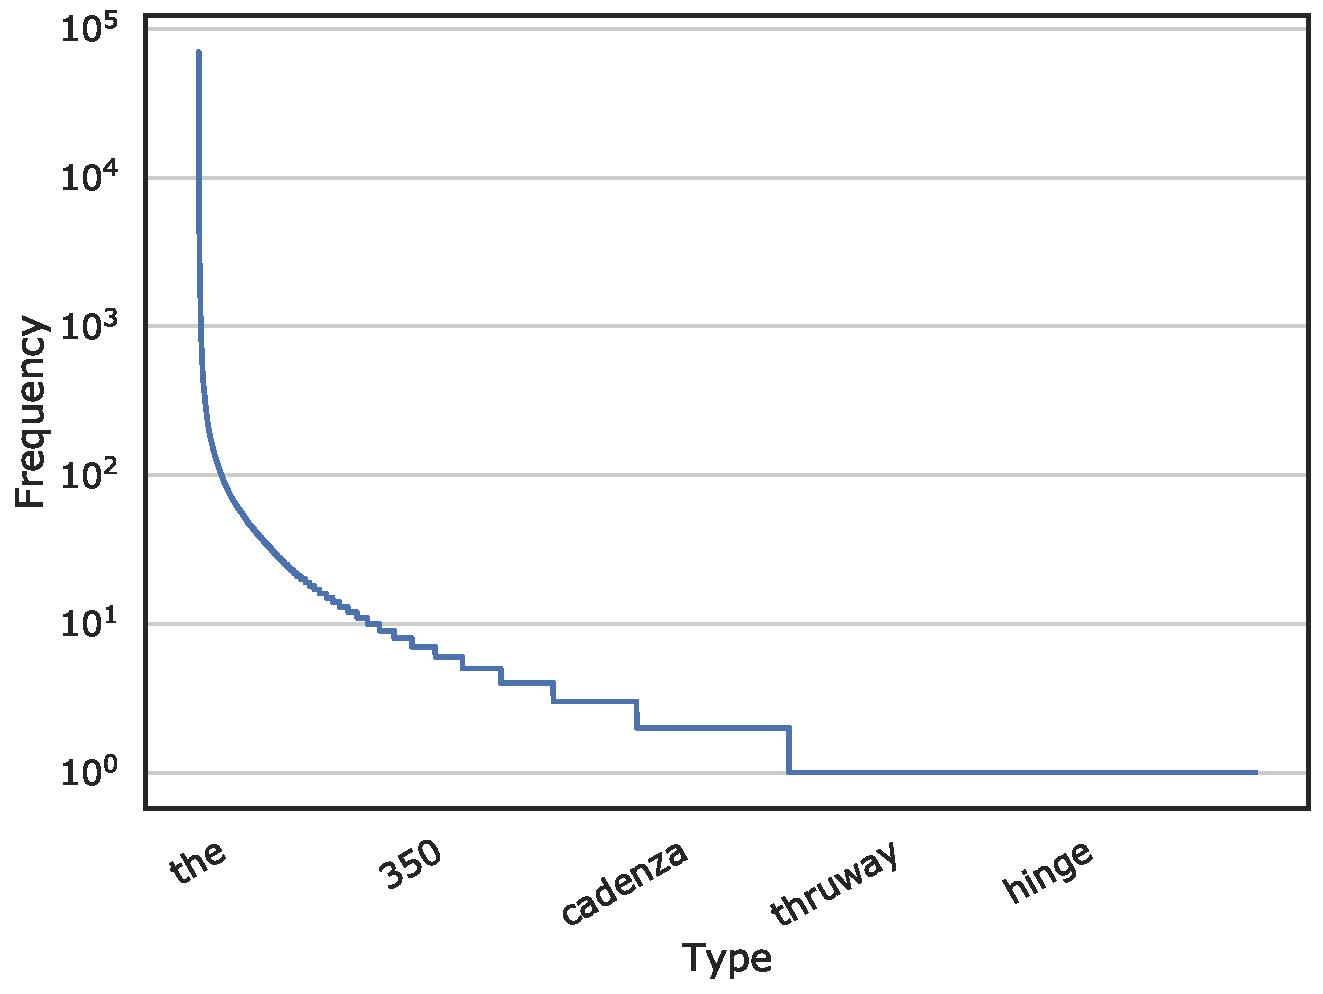
\includegraphics[width=\textwidth,trim={0 0 10mm 8.8mm}, clip]{img/background/brown-corpus-zipf.pdf}
    \caption{Word type frequencies}
    \label{fig:brown-freqs}
    \end{subfigure}
    \begin{subfigure}[t]{0.49\linewidth}
    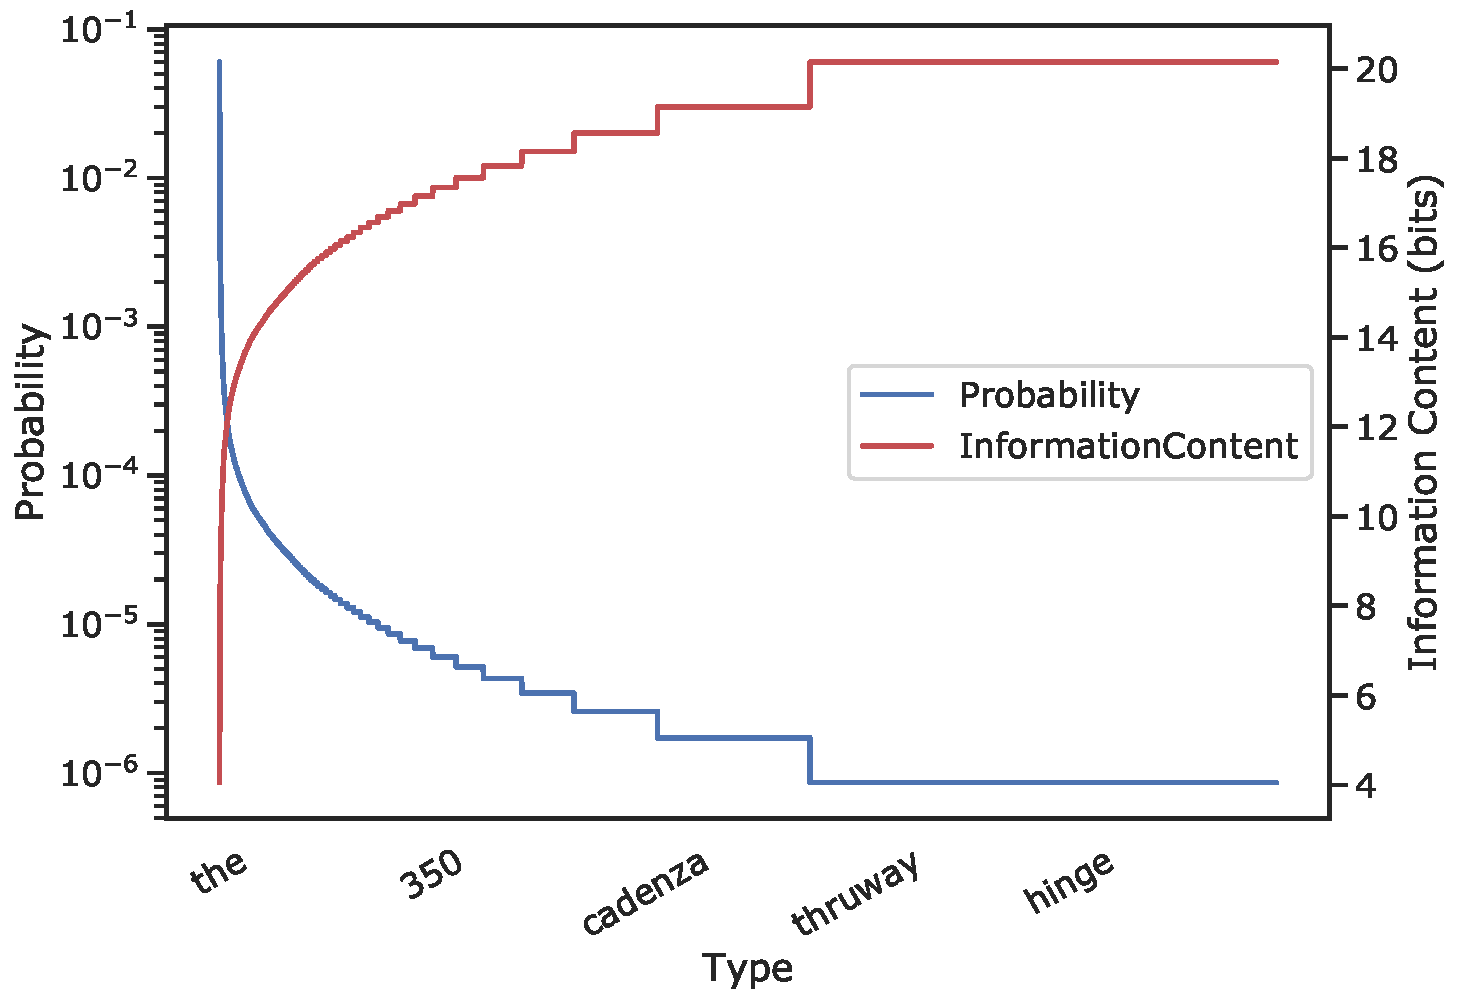
\includegraphics[width=\textwidth,trim={0 0 0 8.8mm},clip] {img/background/brown-corpus-shannons.pdf}
    \caption{Information content distribution across types}
    \label{fig:brown-shannons}
    \end{subfigure}
    
    \caption{Word type frequencies and information content, as observed in the Brown Corpus \cite{kuvcera1967brown-corpus}, which is retrieved using NLTK \cite{bird-2006-nltk}.}% and re-tokenized with NLTK word tokenizer.}
\end{figure}

%\begin{figure}[ht]
%\centering
%\end{figure}

\noindent \textbf{Thesis Statement:} The need for improved performance on the long tail of rare categories, i.e., rare phenomena learning problem, is ubiquitous across domains and problem types within machine learning.
This problem manifests in several forms in machine translation at both training and evaluation stages: 
(1) rare words at training, 
(2) rare words at evaluation, 
(3) rare linguistic styles such as code-switching, 
and (4) rare languages. 
By addressing these areas, we can improve our ability to build higher quality, more comprehensive models. This thesis describes our efforts at addressing these areas and points to the most important next steps.


\begin{comment}
\hrule{}
On the one hand, machine learning techniques for classification perform subpar on categories that have only a few to no training examples. 
On the other hand, in many naturally occurring distributions, categorical imbalance is inevitable, and rare categories are often of special interest for which high performance is preferred.
Rare phenomena learning problem is ubiquitous across domains and problem types, however, we focus on rare phenomena learning in sequence-to-sequence transduction problem with machine translation as a specific case.
Natural language datasets are inevitably imbalanced, with a few high frequency types and a long tail of rare types \cite{zipf1949human}. 
As visualized in Figure \ref{fig:brown-shannons}, the rare types carry more \textit{information content} than common types \cite{shannon1948mathematical}, hence, correctly translating and generating them is crucial for good translation. 
Recent ML advancements have enabled systems that can produce fluent translations, but the semantic adequacy is often lacking. 
% , almost indistinguishable from the humans' fluency
This is not surprising, as fluency and grammar are primarily the result of high-frequency function words (which ML does well), whereas low-frequency content words are essential for achieving semantic adequacy \cite{morrow-1986-discourse,kestemont-2014-function}.
%\footnote{\citet{steedman-2008-last} states that `\textit{[o]ne day, either because of the demise of Moore’s law, or simply because we have done all the easy stuff, the Long Tail will come back to haunt us.}'}
% In addition to the rare word types, rare phenomena also manifest in other forms as rare languages and rare linguistic styles.
%, shows that rare word types have more \textit{information content} per type than frequent types.
%however, by nature, these low frequency types have only a few to no examples for ML to learn from. 
Therefore, an improved performance on the long tail of rare categories, i.e., rare phenomena learning,  problem, is essential and requires our special attention. 

Within MT task, rare phenomena learning manifests in several forms and at both training and evaluation stages. 
This thesis is an attempt to tackle the problem, and is organized into four sections, as: (1) rare words at training, (2) rare words at evaluation and (4) rare linguistic styles such as code-switching,  and (4) rare languages, which are described in the following sections.
\hrule{} 
\end{comment}

\section*{Rare Words at Training}
MT has several choices for modeling approaches; currently, neural machine translation (NMT) is the dominant paradigm.
In Chapter~\ref{ch:nlg-imbalance}, we show that NMT models, such as  Transformers~\cite{vaswani-2017-attention}, have much in common with classification models, especially regarding data imbalance and frequency-based biases. 
We emphasize that the naturally occurring type-token ratio in natural languages yields an extremely imbalanced class distribution, and show ways to minimize the severity of this data imbalance.
We show that NMT models suffer from frequency based biases resulting from imbalanced distributions, especially, the poor recall for rare types.  
We provide a heuristic for efficiently choosing the optimal vocabulary size.


\section*{Rare Words at Evaluation}
%%%%% Evaluation
% Automatic evaluation metrics are also a crucial component in ML.  Since the automatic metrics are quicker and cheaper than human evaluation metrics, they play a vital role in accelerating ML experimentation. In addition, due to their objectiveness and reproducibility, they offer a way of comparing and ranking ML approaches, so that the best approach can be chosen for real-world deployment. However, these metrics are not free from errors, and not all metrics are applicable at all situations. 

In the context of classification, evaluation metrics can be broadly divided into macro and micro metrics.
The fundamental difference between these two kinds is whether to treat each \textit{instance}\footnote{We use `token' and `instance' interchangeably.} or each \textit{class}\footnote{We use `class' and `type' interchangeably.} equally when aggregating system performance on a held-out dataset.  
When each class has approximately the same number of instances, the distinction between macro- and micro- metrics is unimportant. 
However, the distinction is important when the classes are imbalanced in evaluation datasets, i.e., not all classes have approximately the same number of instances. 
Micro metrics that treat each instance equally, e.g., accuracy, are not suitable on imbalanced class distributions, especially when rare classes' performance is important.
To illustrate this point, consider a binary classification problem having a 95-to-5 imbalance ratio. 
Any model that labels all instances as the majority class achieves 95\% overall accuracy. However, such a metric is useless in practice when performance on a minority class is important. 
Hence, careful consideration is required in such class imbalanced settings.

Although word types in natural languages are imbalanced by nature, many widely used MT metrics treat each token equally. 
As shown in Figure~\ref{fig:brown-shannons-cum}, the most frequent 30\% of word types comprise 95\% token instances, but contribute only a small fraction of information content. 
 The remaining 70\% of classes comprise a mere 5\% of tokens, however, they contain a major portion of the overall information content.
%To achieve 95\% of performance on a metric that has equal emphasis on each type, not just tokens, requires mastering a significantly larger vocabulary. 
%More recently, some MT models have been witnessed to have comparable performance with humans as per some popular metrics. 
Since the automatic metrics currently popular for MT evaluation treat each token equally, they overlook the importance of rare types.
In Chapter~\ref{ch:eval-metrics}, we justify an evaluation metric that treats important tokens as important (i.e., a macro metric). 
%The proposed macro metric is already in use by other data imbalanced scenarios such as information extraction.
We show that the metric has comparable performance with currently used metrics on direct evaluation of translation quality, and is a strong indicator of downstream cross-lingual information retrieval task.
In addition, we find that the current MT models generally have poorer performance on rare types than frequent types.
% a kind of analysis not possible with other evaluation metrics.
% The proposed metric, by accounting for the word type imbalance, achieves strong correlation with downstream tasks.

\begin{figure}[ht]
    \centering
    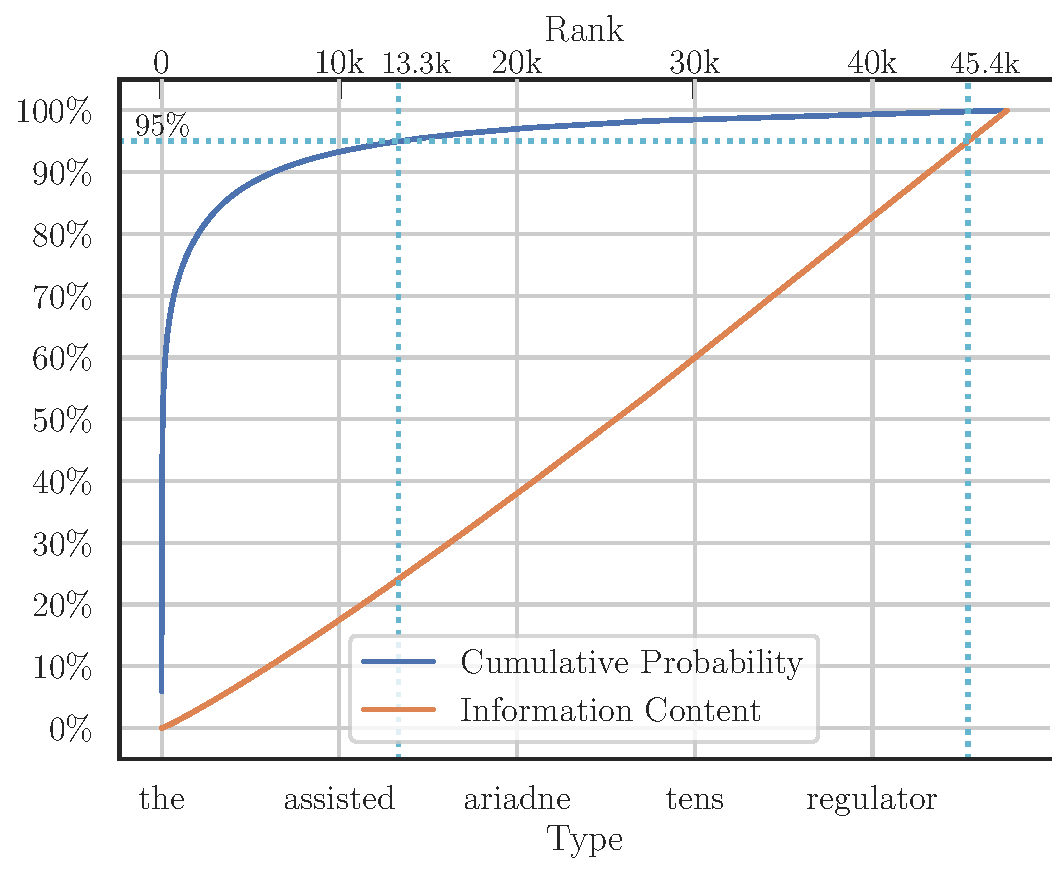
\includegraphics[width=0.6\textwidth] {img/background/brown-corpus-shannons-cum.pdf}
    \caption{Cumulative probability distribution and information content as observed on the Brown Corpus (English) \cite{kuvcera1967brown-corpus}.
    Generation of 95\% of tokens require learning the top 30\% of types only. 
    However, much of the information  content is in the remaining 70\% types, which yield only 5\% of tokens in the corpus.}
    % , to aim for 95\% of \textit{information content} in a language system require learning the 95\% of its types.
    \label{fig:brown-shannons-cum}
\end{figure}


\section*{Rare Linguistic Styles: Language Alternation}
%Multilingual translation models are efficient and practical solution for suporting many languages.
We have multilingual MT models that can translate from hundreds of languages, but they are not as robust as human translators.
An interesting phenomenon in multilingual settings is language alternation (also known as code-switching), in which speakers seamlessly alternate between two or more languages in a single context \cite{cms-and-ury-1977-biling}. 
This phenomenon is common among second language learners, bilingual, and multilingual speakers.\footnote{Although the exact statistics are unavailable, it is estimated that more than half of the world's population is bilingual \cite{grosjean-2010-bilingual}. 
In Europe, where better statistics are available, as per 2016's survey by European Union, 66.6\% of people aged 25–64 speak at least two languages and 29.4\% speak three or more. The number of bilinguals and multilinguals has upward trends over the years.} 
%either for the naturalness of phrases or during the (second or target) language acquisition with only a partial competancy has been attained.
For instance, the European Parliament\footnote{\url{https://web.archive.org/web/20220115222202/https://www.europarl.europa.eu/doceo/document/CRE-9-2021-11-10_EN.pdf}}
and the Parliament of India\footnote{\url{https://web.archive.org/web/20220105061052/http://loksabhadocs.nic.in/debatestextmk/17/VII/01.12.2021.pdf}} hold debates in multilingual environments where multilingual speakers frequently alter languages. 
Figure~\ref{fig:example-langswitch} shows an example of language alternation.
While multilingual human translators can adapt to such an unconventional linguistic styles, in Chapter~\ref{ch:robustness}, we show that multilingual MT models, as currently built, are not robust to such language alternations. In addition, we propose simple methods to evaluate and improve robustness.

\begin{figure}[ht]
    \centering
    \begin{tabular}{ p{0.07\linewidth}  p{0.85\linewidth}}
    \hline
    Original &: {``\textit{Ce moment} {when you start} \textit{penser en deux langues} {at the same} \textit{temps!}"} \\
    \textit{French} & : \textit{``Ce moment quand vous commencez à penser en deux langues au même temps!"}\\
    English & : ``The moment when you start to think in two languages at the same time!"\\
    \hline
    \end{tabular}
    \caption{Demonstration of language alternations between a pair of languages; \textit{French} and English are shown.}
    \label{fig:example-langswitch}
\end{figure}
\begin{figure}[htb]
    \centering
    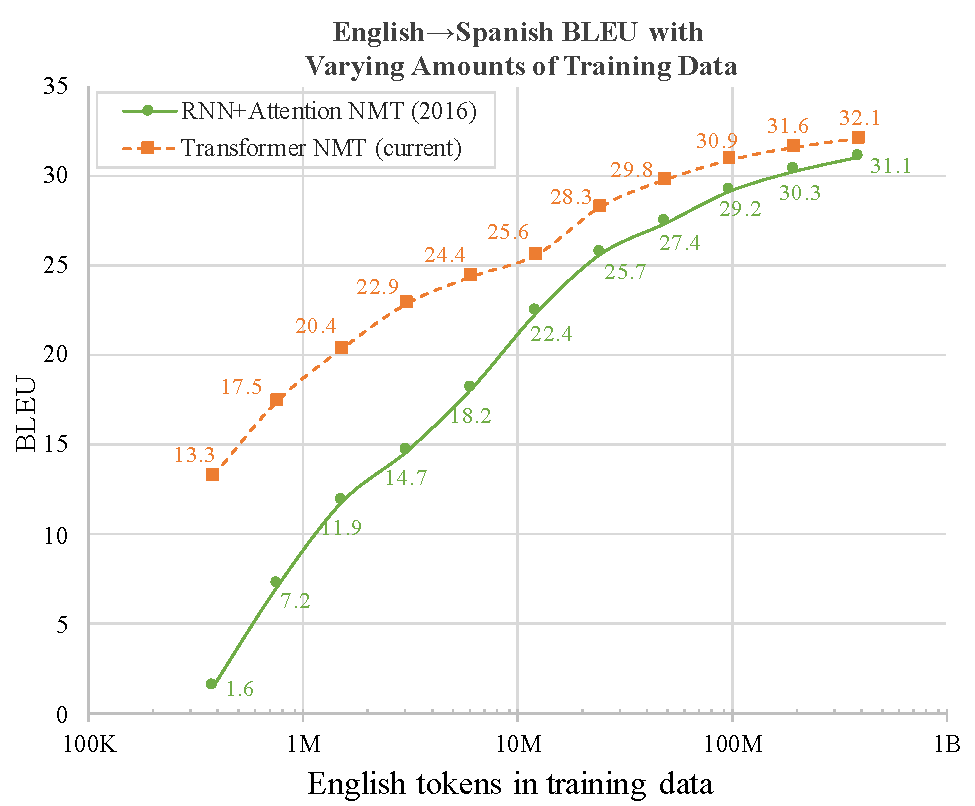
\includegraphics[width=0.65\textwidth] {img/misc/learning-curve-min.pdf}
    \caption{NMT learning curve \cite{koehn2017sixchallenges} revised: the current NMT models produce better quality translations than prior NMT models. The quality improvement is substantial in low resource scenario (left).}
    \label{fig:nmt-learning-curve-min}
\end{figure}


\section*{Rare Languages}
There are at least 7,100 known living languages on our planet \cite{eberhard2019ethnologue}; see Table~\ref{tab:ethn-lang-stats} for a summary of statistics.\footnote{\url{https://web.archive.org/web/20190401105648/https:/www.ethnologue.com/statistics/size}}
The distribution of languages and speakers is also imbalanced. 
Current MT efforts have been targeted to the top hundred languages; there are no readily accessible machine translation systems for thousands of languages.
 % which cover about 85\% of people (~1.5\% of world's languages); (the remaining 15\% of speaker populations from 98.5\% of languages)

In practice, to support translation of rarer languages, three items are essential: (a) efficient translation modeling, (b) powerful computing hardware, and (c) sufficient training data. 
NMT modeling has made considerable progress: the current NMT models achieve better quality than prior generation models in the limited training data settings; see Figure~\ref{fig:nmt-learning-curve-min} for a visualization. 
Computing hardware, especially GPUs, has significantly progressed over the past decade, and enabled the realization of larger and powerful models. 
Therefore, the only missing item in our list is the training data. 
Even though datasets are unavailable for all languages, there exists some quantity of data for at least 600 languages on the web. 
However, since the datasets are at various sources where the formats and naming conventions are not uniform, the curation of datasets into a usable format is a major challenge. 


In Chapter~\ref{ch:rare-langs}, we present a set of tools open-sourced with the aim to advance translation systems for all languages.
These tools greatly simplify tasks such as downloading datasets, storing, and accessing datasets, and training translation models as well as deploying them with web application and RESTful APIs. 
Using these tools, we demonstrate the creation of one of the largest multilingual translation models that supports translating 600 languages to English.

\begin{table}[ht]
    \centering
\begin{tabular}{r : r r r :  r r r}
\hline\hline
\multirow{2}{*}{Population Range} & \multicolumn{3}{c:}{Number of Languages} & \multicolumn{3}{c}{Number of Speakers} \\
& Count & Percent & Cum\% & Total & Percent & Cum\% \\
\hline
100M - 1B & 8 & 0.1 & 0.10 & 2.8B & 40.46 & 40.46 \\
10M - 100M & 86 & 1.2 & 1.30 & 2.8B & 40.00 & 80.47 \\
\hdashline
1M - 10M & 313 & 4.4 & 5.70 & 1B & 14.09 & 94.56 \\
100k - 1M & 977 & 13.7 & 19.50 & 310M & 4.44 & 99.00 \\
10k - 100k & 1,812 & 25.5 & 44.90 & 62M & 0.89 & 99.89 \\
1k - 10k & 1,966 & 27.6 & 72.60 & 7.5M & 0.107 & 99.99 \\
\hdashline
100 - 1k & 1,042 & 14.7 & 87.20 & 0.5M & 0.007 & \multirow{5}{*}{ 100.0 } \\
10 - 100 & 305 & 4.3 & 91.50 & 12k & 0.0002 & \\
1 - 9 & 114 & 1.6 & 93.10 & 465 & 0.00001 & \\
0 & 314 & 4.4 & 97.60 & 0 & 0 & \\ \hdashline
Unknown & 174 & 2.4 & 100.0 & & & \\
\hline
Total & 7,111 & & & 7B & & \\
\hline
\end{tabular} 
\caption{Language and speaker statistics. Source: Ethnologue \cite{eberhard2019ethnologue}.} 
% Source: https://web.archive.org/web/20190401105648/https:/www.ethnologue.com/statistics/size
\label{tab:ethn-lang-stats}
\end{table}

\section*{Overview}
In this dissertation, we attempt to address rare phenomena learning in the sequence-to-sequence transduction problem, with machine translation as a specific case. We present our findings in the following order:
% In Chapter \ref{ch:affirmative-action}, we philosophize imbalance learning as \textit{going the extra mile} in favor of minority categories, whose parallel counterpart in the social sciences is called \textit{affirmative action} (AA), and discuss its ethical implications. 
In chapter \ref{ch:ml-background}, we review the machine learning background material required to understand the subsequent chapters. 
In chapter \ref{ch:nlg-imbalance}, we focus on NMT and show the consequences of imbalance on modeling decisions. We show that NMT models have undesirable frequency-based biases; a notable bias is poor recall of rare types. 
In chapter \ref{ch:eval-metrics}, we show that currently used evaluation metrics ignore the word type imbalance, and some new ones proposed are biased and opaque; we present an interpretable evaluation metric that treats important words as important.
%\tg{In Chapter \ref{ch:imb-learning}, we study both the methods and our proposed methods for machine learning from imbalanced categorical distributions.Here we consider NMT as a complex classification task, we start with simple classification tasks such as image classification, text classification and build our way to the NMT task.}
In chapter \ref{ch:robustness}, we explore methods to measure and improve NMT robustness to rare linguistic styles such as language alternation and partially translated inputs.
In chapter \ref{ch:rare-langs}, we present tools for scaling NMT to rare languages. 
By applying our simplified view of NMT as multi-class classifier, we develop a many-to-one translation model.
While the current multilingual NMT efforts are limited to 100 languages, we expand translation support to 500 languages on the source side (i.e., 400 extra rare languages). 
In chapter \ref{ch:related-work}, we discuss related work. 
Finally, we provide a conclusion and discuss future directions in chapter \ref{ch:discussion}. 

\begin{comment}
\noindent\rule{\linewidth}{1pt}
\section*{Contributions}
\begin{enumerate}
    \item \textbf{The inevitable long-tail curse: Rare words at training:} Most of the information of a language system is in rare words, but these high information \textit{rare} words have only a few, and often zero, training examples to learn from.  While completely resolving this curse may be impossible, I'll show that it is possible to mitigate the severity by adjusting a few hyperparameters during the modeling phase.
    
    \item \textbf{Rare words at evaluation:} I show that widely used MT evaluation metrics do not address the inevitable imbalance in word type distributions. As a result, they place more emphasis on stopwords and overlook rare words. I propose using a simple metric that addresses word type imbalance, and show that it is effective in direct assessment as well as indirect evaluation on downstream tasks. 
    
    \item \textbf{Rare languages: scaling NMT to 500 languages:} I discuss my efforts to expand MT support to low-resource languages currently unsupported by others. I showcase a single NMT model that can translate from 500+ languages to English. 
    
    \item \textbf{Robustness of multilingual NMT:}  Multilingual speakers can and do seamlessly switch languages, whereas multilingual machine translators, as built currently, are not robust to such sudden changes. I propose techniques to measure and improve the robustness to language switching of multilingual translators. 

\end{enumerate}


%Artificial intelligence (AI), powered by machine learning (ML), is transforming the world we live in today. 
%AI and ML applications which were previously limited to constrained environments are nowadays widely deployed in almost every field in the wild. 
%ML techniques are broadly classified intro two categories based on the nature of output random variable.
%Firstly, classification models deal with discreet random variables and hence model categorical distributions. 
%Lastly, regression models deal with continuous random variables hence model continuous distributions.
%Machine learning (ML) has numerous applications; e.g., spam email detection, cancerous tumor detection, fraudulent transaction detection, text sentiment analysis, image classification, named entity recognition, and information extraction.
Machine learning (ML) models are usually studied under balanced categorical distributions.
% ; the datasets curated and used by academia also have balanced categories
%\footnote{Many text classification datasets made accessible via huggingface-datasets, tensorflow-datasets and torchtext are purposefully balanced: e.g. even though DBpedia ontology classes are imbalanced in nature, the commonly used DBpedia-14 dataset is balanced.},
%e.g., SNLI \cite{maccartney-manning-2008-snli}, Sentiment Classification (IMDb reviews) \cite{maas-etal-2011-imdbreview}, MultiNLI \cite{williams-etal-2018-multinli}, XNLI \cite{conneau-etal-2018-xnli}, CIFAR-\{10,100\} \cite{Krizhevsky-2009-CIFAR}, nearly balanced, e.g. MNIST \cite{lecun1998-mnist}.
However, naturally occurring categorical distributions are often imbalanced. 
In many real-world settings, imbalance is inevitable, e.g., fewer cancerous patients than non-cancerous, fewer fraudulent transactions than legit.
In some scenarios balancing is impossible; e.g., image segmentation problem has more background pixels than the foreground pixels, natural language word types are always imbalanced.
An imbalanced categorical distribution results in the formation of majority and minority categories.
\footnote{The terms \textit{majority} and \textit{minority} may sometimes be referred to as \textit{frequent} and \textit{rare}, respectively. The term \textit{category} is referred to as \textit{class} in the context of machine learning, 
% as \textit{group} in social sciences, \textit{symbol} in symbolic communication systems,
and as \textit{type} in the context of natural language processing.} 
Even though the minority categories do not have many training examples in the real world datasets, they are often the interesting find and hence cannot be ignored. 

When ML techniques such as classification modeling are applied on imbalanced distributions without accounting for the inevitable imbalance, we face the following two problems:
\begin{enumerate}
\item There exist noticeable performance difference between majority and minority categories. 
% The difference varies based on the level of imbalance. 
Classifiers achieve higher performance (usually quantified using Precision, Recall, F-measure) on the majority classes whereas relatively poor performance on the minority classes. 
Sometimes this phenomenon is attributed to frequency-based biases in modeling.
% minority classes suffer from under-recall, hence poor recall, and the majority classes suffer from over-recall, hence poor precision.

\item Evaluation metrics that do not account for categorical imbalance may overlook performance on minorities.
They might give false sense of confidence on system performance. 
To illustrate this, consider a binary classification problem having an imbalance ratio of 99:1. 
Any model that assigns a majority class label to all instances easily achieves 99\% overall accuracy. However, such a model is useless in practice.
\end{enumerate}


%\textcolor{gray6}{
Though the imbalanced categorical distributions are common in almost every domain, the efforts towards learning from imbalanced distributions is mostly targeted a few domains.
With deep learning becoming the mainstream machine learning paradigm, the boundaries between different kinds of tasks are favorably blurred: models are borrowed from one domain to other: CNN models which were originally used for computer vision have also proved effective in natural language processing (NLP), and the Transformer models which were originally used for NLP tasks have also proved effective in computer vision tasks.
Hence, we believe the findings on imbalanced learning can also be transferred from one domain to the other, however it is not formally verified before.
In this work, we take the lessons learned from tasks where imbalanced learning is well explored and apply to the areas such as natural language generation where the efforts are scant.




%\begin{figure}[ht]
%    \centering
%    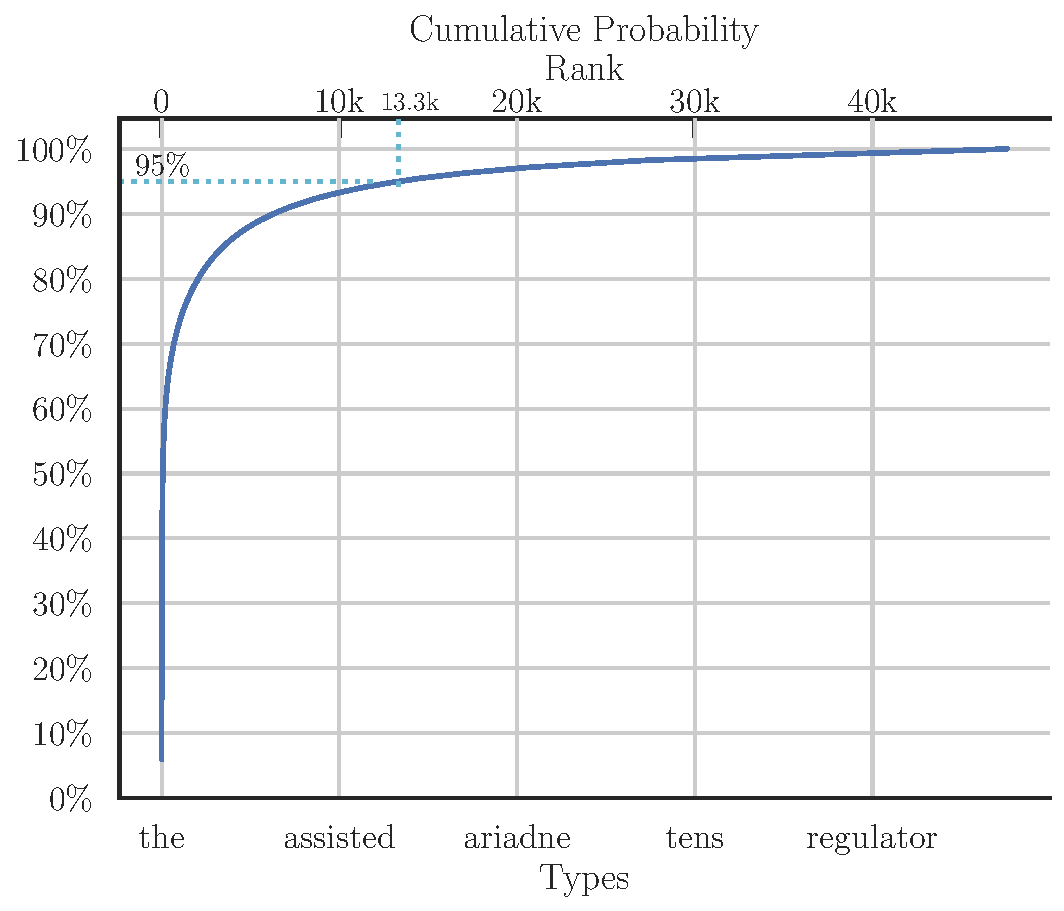
\includegraphics[width=0.5\textwidth] {img/background/brown-corpus-zipf-cum.pdf}
%    \caption{Brown Corpus Cumulative}
%    \label{fig:brown-prob-cum}
%\end{figure}

\end{comment}

